% !TEX encoding = UTF-8
% !TEX TS-program = pdflatex
% !TEX root = ../tesi.tex

%**************************************************************
\chapter{L'azienda}
\label{cap:processi-metodologie}

\section{Profilo}
Web PD s.a.s. é una software house nata nel 2009, con sede a Padova ma con clienti in tutta Italia. La società nasce con lo scopo di gestire portali ecommerce, ma negli anni ha modificato la sua key activity in sviluppo di soluzioni software personalizzate. Ad oggi si occupa di consulenza informatica su software gestionali, applicazioni web e mobile (sia Android che iOS).\\
\begin{figure}[!h] 
	\centering 
	
\includegraphics[width=0.4\columnwidth]{azienda/logo_webpd} 
	\caption{Logo WebPD}
\end{figure}
\\
Il primo prodotto realizzato da Web PD é il gestionale Martina, un software per piattaforma Windows, sviluppato secondo un’architettura client-server modulare, che consente la gestione del ciclo attivo (vendite) e passivo (acquisti) di un’impresa commerciale. Grazie alla sua struttura modulare, é possibile aggiungere a Martina diverse funzionalità, come ad esempio gestione di magazzino, gestione della contabilità e
gestione dello scadenziario.\\
\\
Successivamente l’azienda aggiunge al portfolio di servizi offerti anche la realizzazione, grazie alle piattaforme OpenCart e Prestashop, di siti e-commerce integrati al gestionale Martina. \\
È in questo contesto che prima nascono gli ecommerce TuttoNauticaWeb.com e MiglioNautico.com, successivamente FarmaZero.com e SubitoStore.com.\\
\\
Nel 2015 Web PD da s.a.s. si trasforma in s.r.l. perché ha l’intenzione di addentrarsi nel settore turistico; questa strategia si perfeziona con l’acquisizione di un agenzia di viaggi ad Albignasego (PD).\\
\\
Nel 2016 il network e franchising di agenzie di viaggio Primarete Viaggi e Vacanze s.r.l. acquisisce il 49\% delle quote sociali di Web PD s.r.l.. Il frutto di questa collaborazione é l’ammodernamento, continuo ed ancora in corso, dei portali Viaggiregalo.it, CrociereRegalo.it, SimaWorldTravel.it e PercorsiReligiosi.it, di proprietà di Promoter Travel s.r.l., una controllata di Primarete.\\

\section{Dominio tecnologico}
L'azienda offre un ampio ventaglio di prodotti, che coinvolgono diverse piattaforme. È opportuno esaminare le tecnologie adoperate raggruppandole nelle seguenti categorie: \textit{Web}, \textit{Mobile} e \textit{Desktop}.

\subsection{Web}
In WebPD, la realizzazione di prodotti basati su piattaforma Web avviene, a livello di backend, utilizzando come linguaggio di programmazione PHP (versione 5 o 7). Molto spesso, per i progetti più complessi, viene usato il framework \textit{Codeigniter} (versione 3), che agevola l'implementazione del design pattern MVC e fornisce numerosi strumenti per facilitare (dunque accellerare) lo sviluppo. Codeigniter, tra le altre cose, infatti, implementa una serie di classi che facilitano l'esecuzione ed il debug delle query, oltre ad un meccanismo che permette di salvarle in cache (aumentando notevolmente le prestazioni del prodotto).\\
\begin{figure}[!h] 
	\centering 
	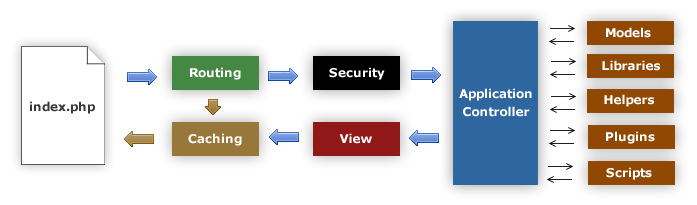
\includegraphics[width=1.0\columnwidth]{azienda/codeigniter_flow} 
	\caption{Flow chart di un'applicazione creata con Codeigniter}
\end{figure}\\
Per quanto riguarda il frontend, invece, viene utilizzato HTML5, CSS3 e Javascript (jQuery), senza usare framework che implementino Single Page Application (come React.js o Angular).\\\\\
Come server web, infine, vengono usati \textit{Apache2}, in caso di hosting su piattaforma Linux, o  \textit{IIS}, in caso di hosting su piattaforma Windows.\\\\
Per la realizzazione di siti web semplici, dove per semplici si intende senza esigenze di svolgimento di operazioni complesse, viene prediletto l'utilizzo di CMS, quali Wordpress (nel caso di blog, vetrine o forum) e OpenChart (nel caso di siti di e-commerce).
\\
\\
\subsubsection{DBMS}
Per lo sviluppo di prodotti software, WebPD si appoggia a due DBMS: \textit{Microsoft SQL Server 2012} e \textit{MySQL Server}. Entrambi questi software sono RDBMS, ma la scelta di utilizzare l'uno o l'altro dipende dalle caratteristiche del progetto, nello specifico: \begin{itemize}
	\item \textbf{Microsoft SQL Server} viene utilizzato nei progetti che prevedono un'ampia mole di dati da gestire e interrogazioni (query) complesse (come, ad esempio, CrociereRegalo.it), in quanto in tali contesti si è dimostrato mediamente più performante di \textit{MySQL};
	\item \textbf{MySQL Server} viene utilizzato il più possibile in caso il progetto non contenga una grossa mole di dati e/o interrogazioni complesse, in quanto non prevede costi di licenza (mentre \textit{SQL Server} si, e anche abbastanza elevati \footcite{site:sql-server-pricing}) ed é multipiattaforma (attualmente disponibile per Linux, Windows e MacOS).
\end{itemize}

\subsection{Mobile}
Il know-how accumulato da WebPD nella realizzazione di applicazioni web ha portato all'adozione del framework \textit{Cordova} per la creazione di applicazioni mobile, il quale offre la possibilità di creare app ibride cross platform utilizzando HTML/CSS e Javascript. Tali applicazioni, grazie ad alcune interfacce messe a disposizione da Cordova, possono accedere alle funzionalità native del dispositivo, come fotocamera, storage o sensoristica varia (accellerometro, giroscopio e GPS, se presenti).

\begin{figure}[!h] 
	\centering 
	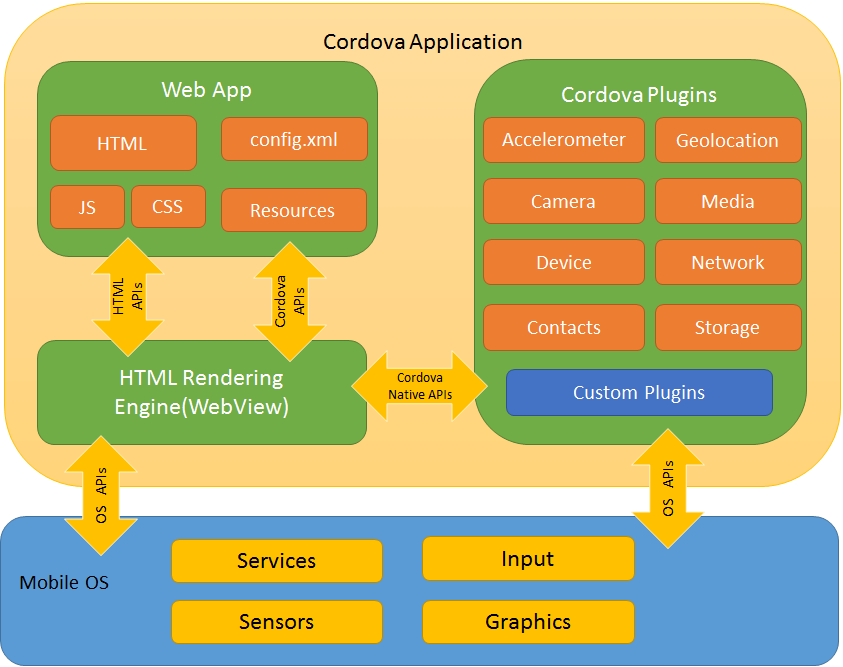
\includegraphics[width=0.6\columnwidth]{azienda/cordova_architettura} 
	\caption{Schema dell'architettura di un'app basata su Cordova}
\end{figure}

\subsection{Desktop}
La realizzazione di applicazioni desktop avviene attraverso l'utilizzo di due linguaggi: Java e Delphi.\\
Delphi viene usato soprattutto quando i programmi necessitano di manipolare grandi basi di dati, in quanto le applicazioni sono compilate in binario, quindi mediamente più performanti, e il linguaggio possiede numerose librerie che ne facilitano l'accesso.\\
Java, di contro, viene usato quando si ha l'esigenza di creare applicazioni cross-platform che non coinvolgano grandi volumi di dati.

\section{Processi aziendali}
\subsection{Ciclo di vita}
In WebPD, la \textit{way-of-working} inerente al ciclo di vita del software aderisce al \textit{modello Evolutivo}.\\
L'adozione di tale modello deriva (principalmente) dall'esigenza di dover adattarsi alla mutevolezza dei requisiti. È un dato di fatto, purtroppo, che molto spesso neanche il cliente stesso sa di preciso che cosa vuole, quindi solo "toccando con mano" l'istanza del suo pensiero esso sa dire se effettivamente è quello che fa per lui o no.\\
\begin{figure}[!h] 
	\centering 
	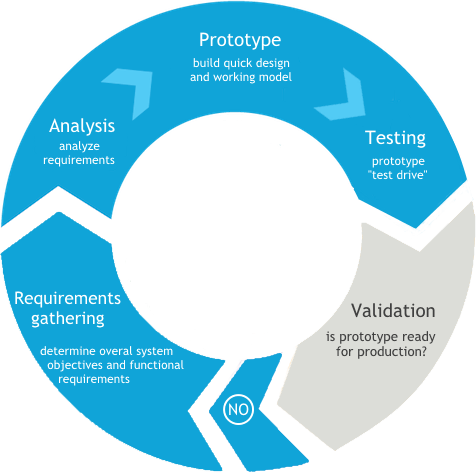
\includegraphics[width=0.6\columnwidth]{azienda/modello_evolutivo} 
	\caption{Schema del modello evolutivo. URL: \url{https://bit.ly/2N49cUI} }
\end{figure}\\
Questo problema viene affrontato dal modello evolutivo, prevedendo che non venga effettuato solo un unico rilascio, ma che vengano creati prototipi, istanze di un sottoinsieme di requisiti del progetto, sottomessi poi al cliente. L'esito della valutazione dei prototipi può portare ad una rivisitazione dei requisiti inerenti alle funzionalità contenute in essi.\\
Nello specifico, il modello prevede le seguenti fasi :
\begin{enumerate}
	\item \textbf{Analisi e progettazione}, che viene fatta solo all'inizio del progetto e non si ripete;
	\item Per ogni prototipo:
		\begin{enumerate}
			\item \textbf{Progettazione di dettaglio} dei requisiti non implementati;
			\item \textbf{Sviluppo} di quanto appena progettato nel dettaglio;
			\item \textbf{Validazione} del prototipo appena sviluppato e, in base ai feedback del cliente, un'eventuale \textbf{revisione dei requisiti}.
		\end{enumerate}
	\item \textbf{Rilascio} della versione finale, corrispondente all'ultimo prototipo accettato dal proponente.
\end{enumerate}
Il modello evolutivo, inoltre, prevede la possibilità di avere più canali di sviluppo (ad esempio stabile, alpha, beta ecc.), utili per poter "sperimentare" nuove funzionalità senza andare ad intaccare la versione stabile del software.\\
Il problema principale di questo modello è che i tempi di sviluppo possono allungarsi notevolmente. La validazione da parte del cliente, infatti, è un'operazione che può richiedere molto tempo, durante il quale lo sviluppo non può proseguire. Inoltre, in caso di un cliente molto "indeciso", il numero di prototipi può aumentare in modo esponenziale, rischiando quindi che gli \glspl{incremento} si trasformino in \glspl{iterazione}.

\subsection{Miglioramento della qualità dei processi}
Nella way-of-working aziendale è presente una forte attenzione alla qualità dei processi. L'organizzazione interna di questi ultimi è incentrata sul principio del miglioramento continuo, grazie all'applicazione del Ciclo di Deming, conosciuto anche con l'acronimo PDCA. Tale acronimo contiene le iniziali delle quattro fasi in cui è possibile suddividere il processo di miglioramento: \begin{enumerate}
	\item \textbf{Plan}, ovvero pianificare, prima dell'inizio del processo, attraverso una attenta analisi di esso, eventuali problematiche e azioni di miglioramento;
	\item \textbf{Do}, ovvero eseguire il processo monitorato agendo secondo quanto pianificato nella fase precedente;
	\item \textbf{Check}, ovvero valutare (in modo retrospettivo) l'esito delle azioni derivanti da quanto pianificato all'inizio;
	\item \textbf{Act}, ovvero agire standardizzando ciò che è andato a buon fine e correggendo le carenze.
\end{enumerate}
\begin{figure}[!h] 
	\centering 
	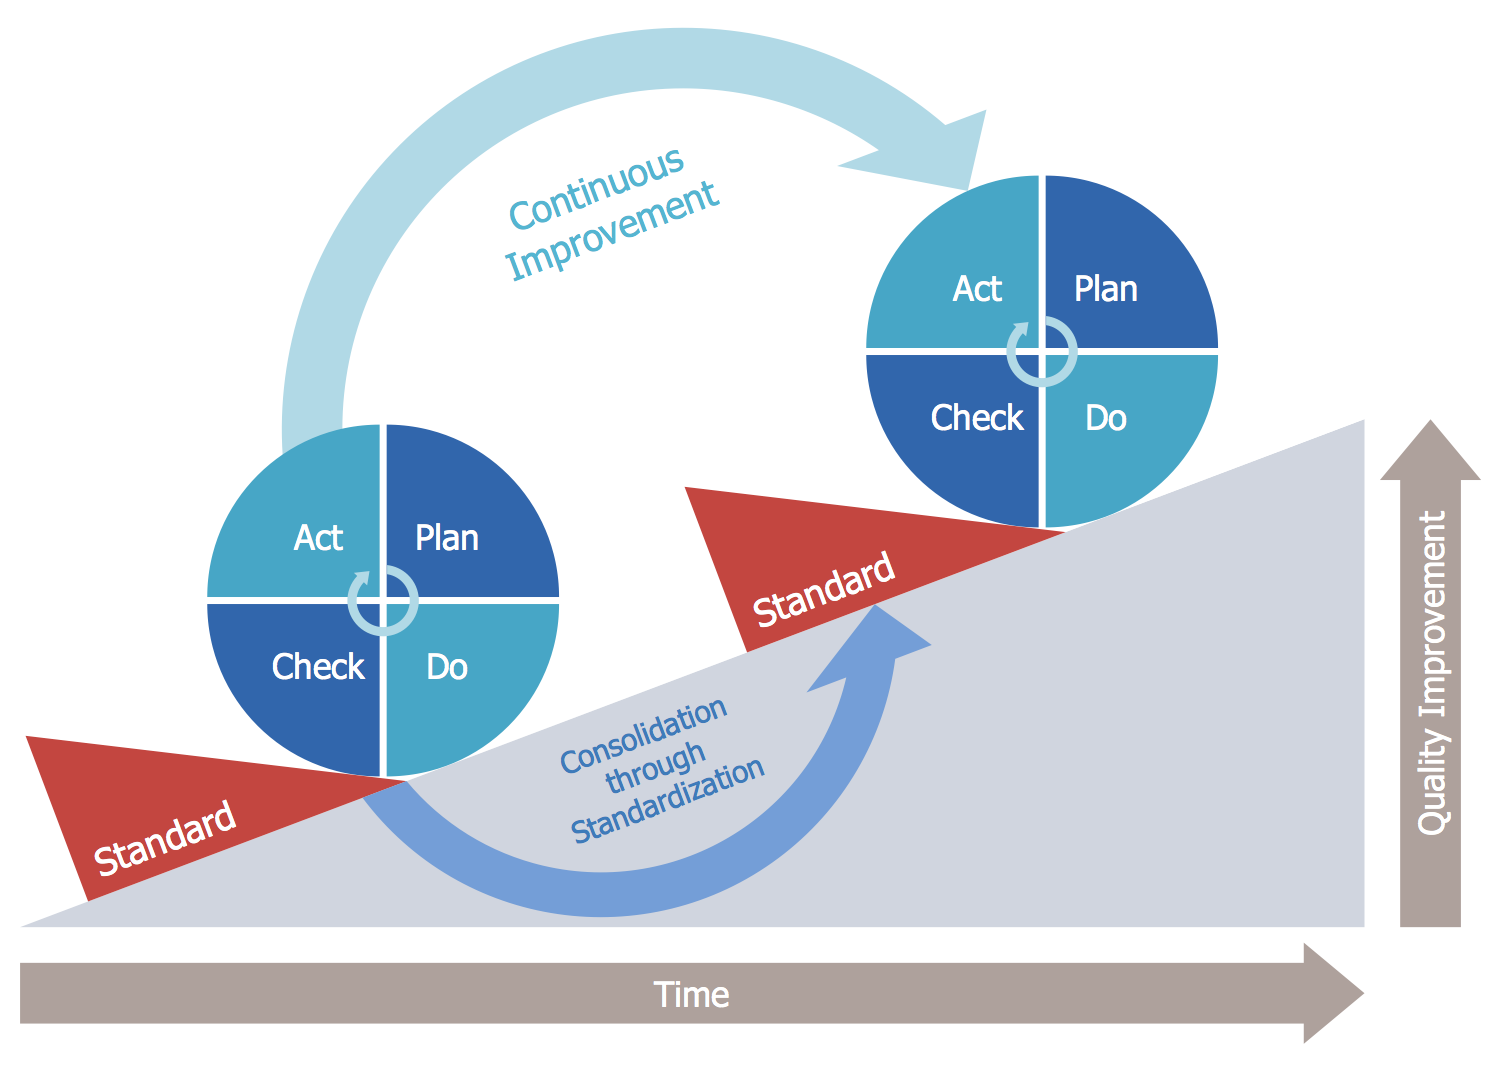
\includegraphics[width=0.6\columnwidth]{azienda/pdca} 
	\caption{Rappresentazione grafica del PDCA. URL: \url{https://bit.ly/2LP32TF} }
\end{figure}
A livello grafico, il PDCA è rappresentato attraverso un cerchio in movimento, che dichiara la ciclicità della sua applicazione.\\
In figura lo standard è rappresentato come un cuneo in quanto agisce da limite inferiore per la qualità. L'obiettivo del PDCA è quindi portare sempre più in alto la qualità dello standard.

\subsection{Strumenti a supporto dei processi}
\subsubsection{Gestione di progetto}
Per quanto riguarda gli strumenti di gestione di progetto, WebPD si affida a \textit{Trello}. 
Trello é uno software di amministrazione di progetto web-based, con tanto di relative applicazioni per Android e iOS. Trello permette la creazione di una bacheca condivisa, organizzata in \textit{cards}, all'interno delle quali é possibile inserire dei compiti da svolgere (\textit{task}) e assegnare ciascuno di questi compiti una data di scadenza. \\
\begin{figure}[!h] 
	\centering 
	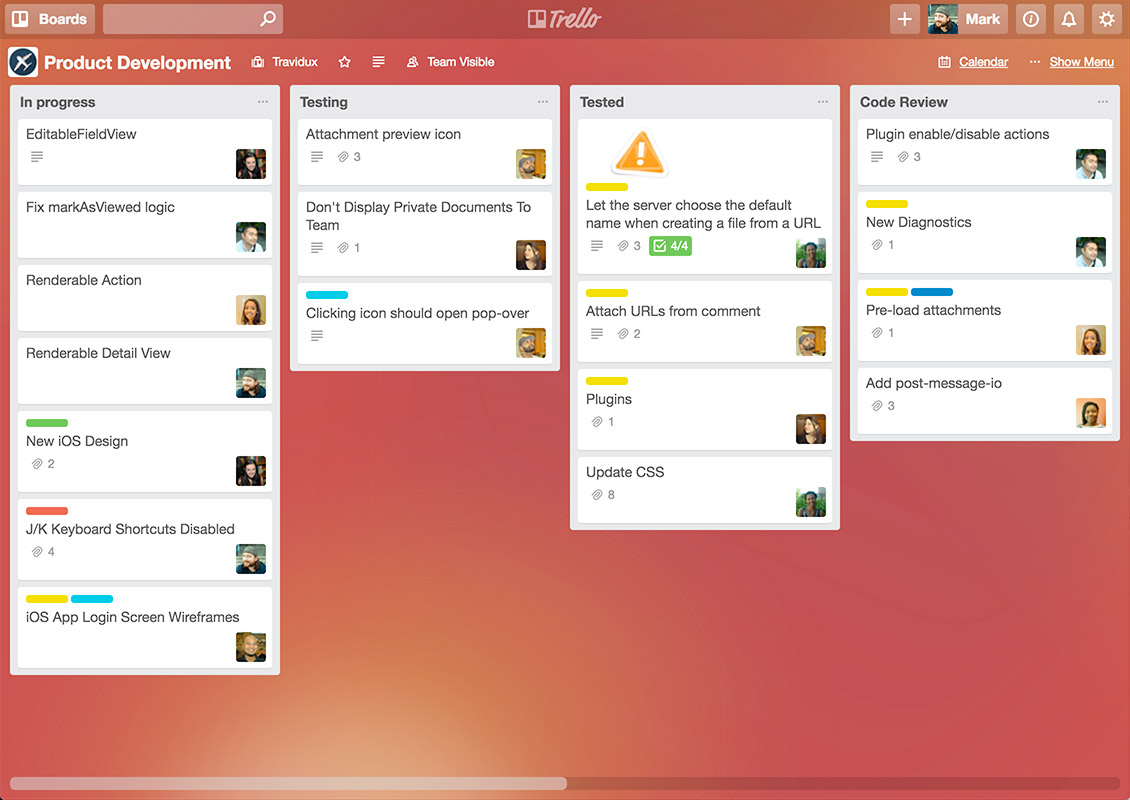
\includegraphics[width=0.8\columnwidth]{azienda/trello} 
	\caption{Screenshot dell'interfaccia web di Trello.}
\end{figure}\\
Su ogni compito é possibile pubblicare dei commenti per, ad esempio, porre domande o fare determinate osservazioni e aggiungere checklist, etichiette (tag) e allegati.\\ 
I \textit{task} possono inoltre essere agilmente spostati tra una \textit{card} e un'altra, funzionalità utile, ad esempio, per tenere quanto più pulita possibile la bacheca, nascondendo i \textit{task} già svolti o raggruppandoli in apposite \textit{cards} aventi funzione di storico.\\
Una feature molto interessante è la sincronizzazione live delle modifiche, che permette a più persone di agire e collaborare sulla bacheca contemporaneamente, senza incorrere nel rischio di visualizzare o modificare dati non aggiornati.\\
Trello, infine, prevede anche numerosi \textit{Power-up}, ovvero estensioni (a pagamento) che permettono di interagire con numerosi servizi, quali, ad esempio, Google Drive, Onedrive, Google Calendar, GitHub, BitBucket, Slack ecc.\\
\\
Per avere una più immediata visualizzazione dell'andamento dei \textit{task}, assieme a Trello viene usato \textit{Trellogantt}. Quest'ultimo, come forse già suggerisce il nome, permette di visualizzare i dati contenuti in una bacheca di Trello sotto forma di diagrammi di Gantt. Inoltre permette, con un semplice drag-and-drop, di modificare le date di scadenza dei vari task.\\

\begin{figure}[!h] 
	\centering 
	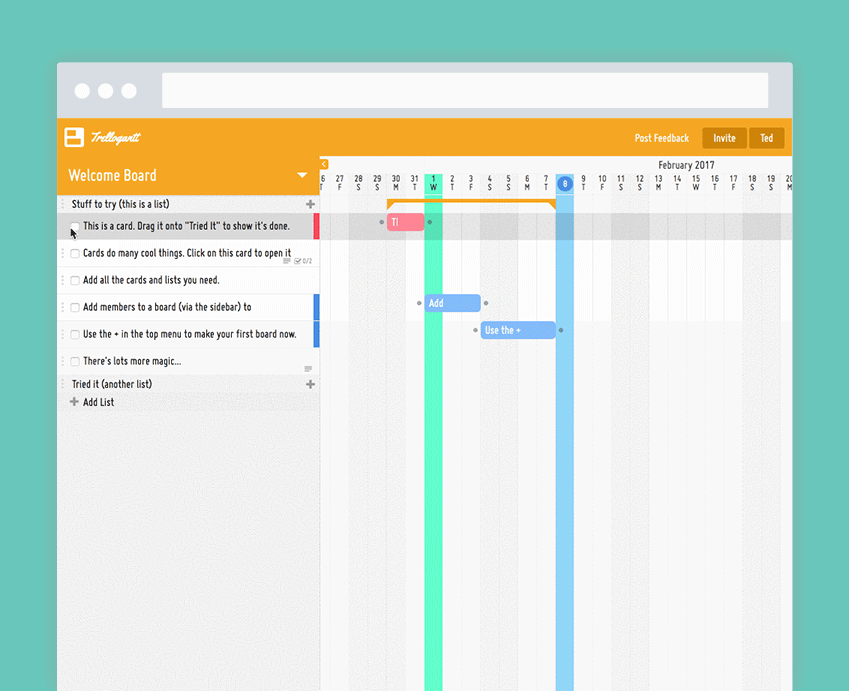
\includegraphics[width=0.8\columnwidth]{azienda/trellogantt} 
	\caption{Interfaccia di Trellogantt. URL: \url{https://bit.ly/2wysjgc} }
\end{figure}


\subsubsection{Gestione di versione}
WebPD, come strumento di versionamento, utilizza il software \textit{Git}, probabilmente il più utilizzato nel suo campo. Le motivazioni che hanno portato all'adozione di Git al posto del suo "antagonista" \textit{Subversion} (SVN) sono le seguenti:
\begin{itemize}
	\item Decentralizzazione del repository: a differenza di Subversion, l'architettura di Git prevede che vi sia una copia dell'intero repository in ciascun client, in modo da poter effettuare \textit{commit} anche in assenza di una connessione verso il server (cosa non possibile con SVN);
	\item Velocità: le operazioni di commit sono molto spesso più veloci su Git in quanto vengono effettuate sulla copia locale del repository, ed é possibile poi inviarle al repository remoto (tramite \textit{push}) in un secondo momento, anche in blocco.
	\item Miglior gestione di branch e tag: in SVN, branch e tag sono copie dell'intero progetto (che quindi possono aumentare molto lo spazio richiesto dal repository sul server), mentre in Git sono semplicemente dei riferimenti ad una determinata commit.
\end{itemize}